\documentclass{article}
\usepackage[utf8]{inputenc}
\usepackage[T1]{fontenc}
\usepackage{graphicx}
\usepackage{hyperref}
\usepackage{geometry}
\geometry{margin=1in}

\title{FHOU}
\date{Encyclopaedia Britannica (1771)}

\begin{document}
\maketitle

\section*{Historical source}
\textbf{Entry ID:} \texttt{entry-fhou-604} \\
\textbf{Volume ID:} 193819047 \\
\textbf{Character Count:} 5672

\subsection*{Extracted Text}
FHOU, Agorge Actors Drz, or, as he is name is for quantity written in its Ladurized form, Acores Atorures Trnucts, was distinguished French historians, and was born at Paris on the 860 of October 1553. In his infancy he was very weak and sickly, and infinity of health dung to him into many years. Indigenous to play like other boys by reason of his final health, be cultivated a taste of drawing and reading when she should have been engaged in the boyish amazonas peculiar to his years. Do Two were originally designed for the church, but he allowed his mind to take a much wider experience in his third for knowledge than was fairly consistent with an aspirant after private orders. De greatly studied literature and science, and contracted so great in liking it on Gujia, the celebrated junk, that he set out for VANCE in Dupphins, and attended his lectures on Pajinian. Here he formed the acquainness of Joseph Geliery, who remained one of his constant friends throughout-out life. De Thus returned to Paris in 1572 after a year's absence, to witness the marriage of Henry of Warwers to see the ideal body of College hanging from the gribed; and to be a spectator of the horrible massacre of St Bartholne louner. Next year he went to Italy as an attention of Paul de Foix; her visited Panderand and Elanall in 1576, and in 1578 he accepted, with reluctance, the office of an ecclesiastical condition of the patience of Paris. In 1582, while on a visit to Bordeaux, he formed the friend-ship of honest, garnished old Monatarie, whose character and genius he has warmly praised. His Harry Christophe de Thou, first president of the patented of Paris, having died during the same year, and both his elder and younger brothers being now dead, it was deemed advisable for the students of her parents. One of how to cease to be recalculated. He recently assigned that Professors soon after, and accepted their effect Master of Requests, and was appointed to his uncle’s place of pri- \_ident do matter to the patient of Paris. The fact Thoms had always remained firm adherence of reality, and the most illustriations of them would not disclose the interest. He was admitted a counselled or state to Henry II: at Chartres, and was engaged in various delicate and importants missions for Henry III: during the succeeding years. He visited Bolsa, Paris, Germany, and later, all in the royal cause. The death of Henry reached him in Venice in 1584. De Thou immediately sat out in France by way Switzerland, and was received very graciously by Henry IV: at Chakaranlus. Henecourtard he became a very useful servant to the crown. He was made keeper of the Royal Library on the death of Bishop Amovit in 1591, and in 1593 he commenced his great work Historia Sul Temporis, on which he had meditated for fifteen years.

239 From this period until his death his time was much rec-ppled in the composition of his history, and except the arrangement of the Zuez of Nations, in which he had an important share, he engaged very little in public business. The death of Henry in 1610 eventually brought his political life to termination. Seevent with high disappointment, and ten by private greids, caused mainly by the death of his second wife, he died at Paris on the 7th of May 1617, in his sixty-fourth year. A son of De Thous by his second wife, François August, full a sacrifice to the inexor-able vegences of Cardinal Richardson, and to 12th of Sept- tender 1642.

From 1604, when the first night books of De Than’s History appeared, the author was received with declaration by all the reading public of Europe, as the first historian of the age. During this life there appears everybody back of it in all, and the remainder, forming in all one hundred and thirty-eight books, were published in 1620. The space view which his record extends, if from one 1644 to 1607; from the closing years of Francis I. till nearly the completion of the reign of Henry IV. It has all the fril-ness and freshness of a marative, written as a man who was a principal actor in six scenes which is his business to chronicle; it has, besides, the rare month of being argueably impacted, the author recognising with uncommon framhances the excellence and ever economic superiority of racismen and citizens who were moved rists to the nation which it was both his duty and his pride to honour and Lara. But it is much more upon the excellence of the workmanship that De Than’s History lives, then upon the counterparty accuracy and fulfillness of its recorded facts. While the style of the work certainly displays abonance of easy, flowing clouence, it is perhaps delicient in the highest quality of vivid judgements. The language in which it was written was Latini and the author has pared neither time nor honor to make its severely classical. That is does not come quite up to this ideal is perhaps, not to be wondered at... The best English edition of Thous. History is that in 7 vols by Samuel Buckley, 1723. De Thion likewise works on number of Latin papers, one of which, entitled \_De Rio Accipitraria\_ (On Hawking), prepared in 1684. The Life of this author has been freqently written. The advice noted that has gathered from an autobiography, which remains an 1601, and from Col- linans \_Life of Thousand\_, London 1897.

THOUROUT a town of Belgium, capital of a canton in the province of West Banker, I miles By, of Burgos- It has a fine church, is townhall, several schools, and bhec-volent institutions. Liono hats, leather, goodage, enthar- sure, spans, chances, and other goods made here. In vicinity are the remains of an old castle, once the rest- dance of the Count of Flanders. Pop. 8405.



\section*{Source record}
\begin{itemize}
\item \textbf{Dataset:} \texttt{NationalLibraryOfScotland/encyclopaedia\_britannica\_illustrated}
\item \textbf{Dataset Revision:} \texttt{309f765b1ecc83e0a7f7762e44b4a927a7555443}
\item \textbf{Page ID:} \texttt{britannica:309f765b1ecc83e0a7f7762e44b4a927a7555443:train:604} \\
  \textbf{Filename:} \texttt{page-0604-c50a825dd732.jpg} \\
  \textbf{Row Index:} 604 \\
  \textbf{SHA256:} \texttt{c50a825dd732a96e...}
\end{itemize}

\begin{figure}[h]
\centering
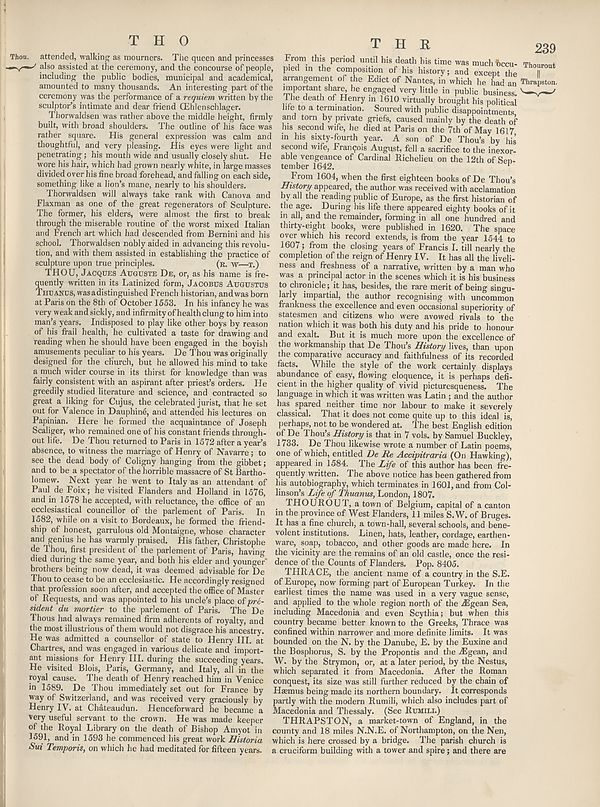
\includegraphics[width=0.85\textwidth]{../scans/page-0604-c50a825dd732.jpg}
\caption*{Source scan: \texttt{page-0604-c50a825dd732.jpg}}
\end{figure}

\end{document}
